\chapter{Spring Data JPA}

\fcolorbox{black}[HTML]{E9F0E9}{\parbox{\textwidth}{%
\noindent \textbf{Learning goals}\\
The junior-colleague
\begin{enumerate}[nolistsep]
\item can describe the concept of ORM.
\item can explain what JPA is, and what it’s not.
\item can denominate different JPA providers.
\item can describe what a persistence unit is.
\item can explain the fundamental interfaces of JPA.
\item can explain what the persistence context is.
\item can implement entity classes.
\item can describe the entity objects’ lifecycle.
\item can implement different types of relationships between entity classes.
\item can implement CRUD operations.
\item can implement queries.
\item can implement named queries.
\item can explain, identify and solve the N + 1 query problem.
\end{enumerate}}}

  
\section{What is ORM?}

Object-Relational Mapping (ORM) is a technique that lets you query and manipulate data from a relational database using an object-oriented programming language.

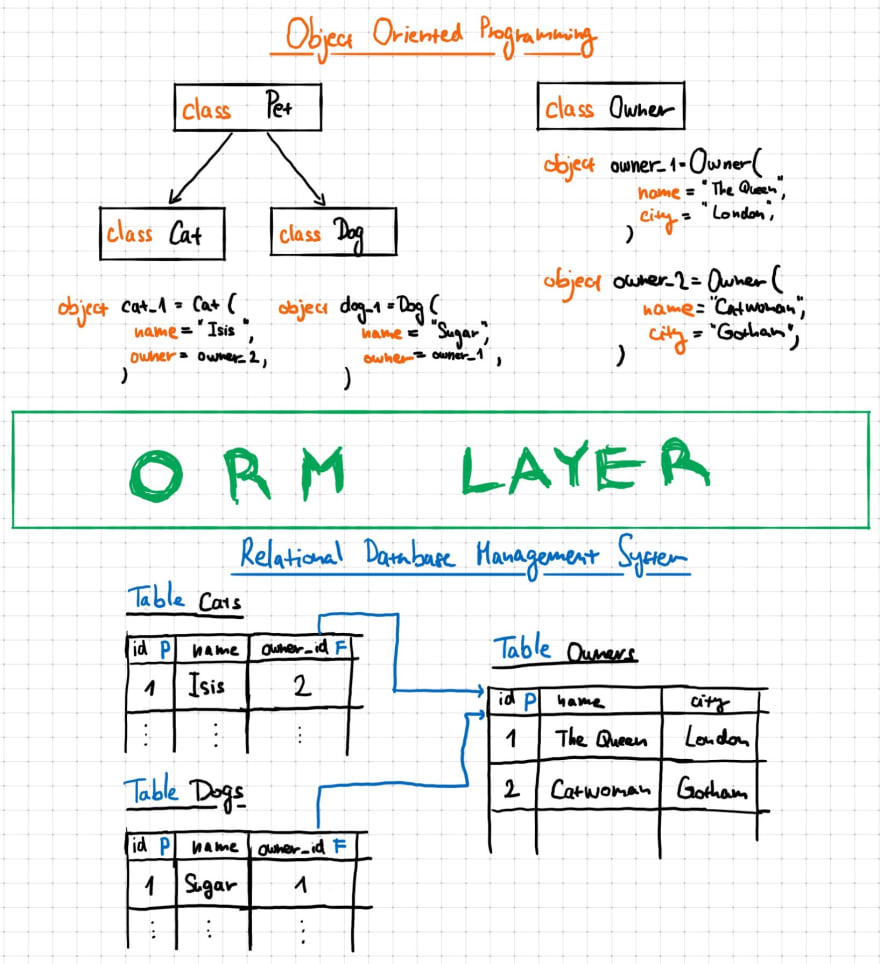
\includegraphics[width=\textwidth]{./images/chapter6/orm}


\section{What is JPA?}

The Java Persistence API (JPA; recently renamed to Jakarta Persistence API) is a specification that defines how to persist data in Java applications. JPA mainly focuses on the ORM layer and managing persistent objects.

JPA is a specification which means JPA consists of implementation guidelines for the Java ORM layer and the syntax. The specification only comes with interfaces, no actual implementation.  A reference implementation can be provided but other companies can create and distribute their own implementation of the specification.

\frame{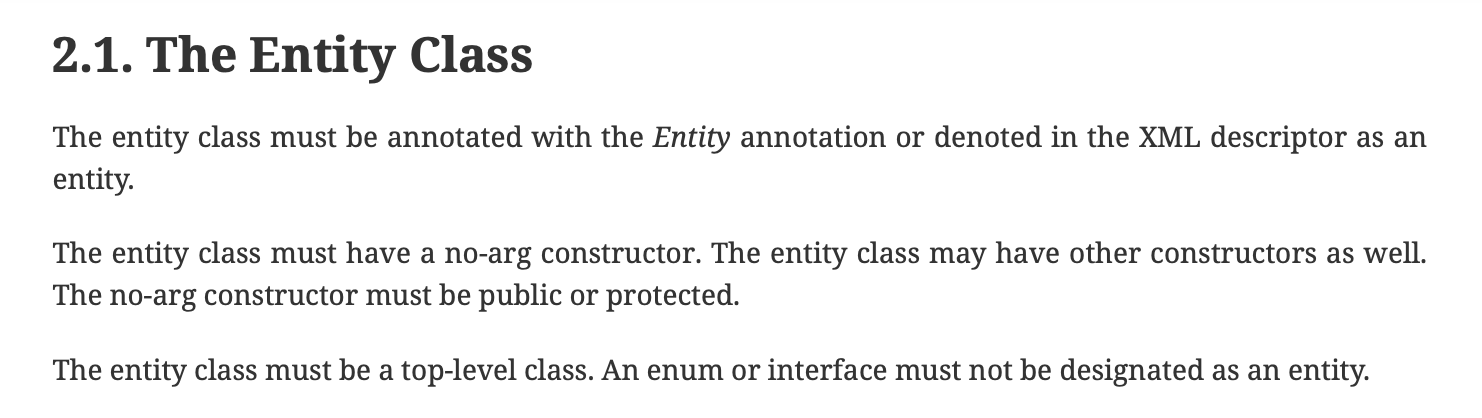
\includegraphics[width=\textwidth]{./images/chapter6/entity_class_specification}}

For our exercises and projects we will use Hibernate as the actual implementation of de JPA specification \footnote{\url{https://hibernate.org/ and https://hibernate.org/orm/}}.  

Spring Data JPA adds a layer on top of JPA. It uses all the features defined by the JPA specification, but adds no-code implementation of the repository pattern and the creation of database queries from method names.

The JpaRepository interface is an extension of CrudRepository.
JpaRepository extends PagingAndSortingRepository which in turn extends CrudRepository.

Their main functions are:

\begin{itemize}
\item CrudRepository mainly provides CRUD functions.
\item PagingAndSortingRepository provides methods to do pagination and sorting records.
\item JpaRepository provides some JPA-related methods such as flushing the persistence context and deleting records in a batch.
\end{itemize}


\section{Datasource}

In Spring Boot a DataSource-object is the preferred means of getting a connection to a database.
The interface jakarta.sql.DataSource is implemented by the database driver vendor. 

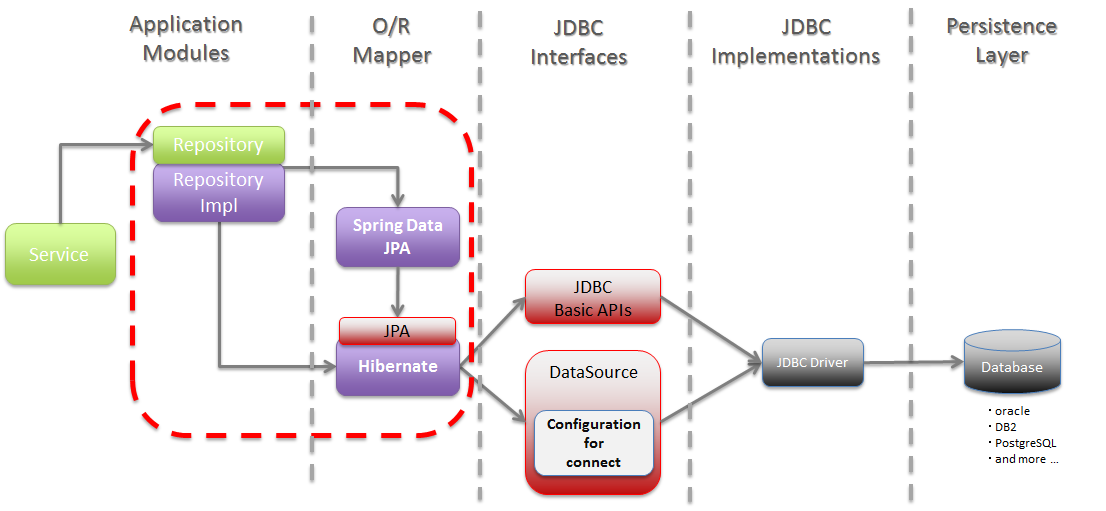
\includegraphics[width=\textwidth]{./images/chapter-jpa/springdatajpa}

The datasource can be specified in the application.properties file.
Here are some common database properties:

\begin{tabular}{|l|p{8cm}|}
\hline
spring.datasource.url & JDBC URL of the database.\\
spring.datasource.username & Login username of the database.\\
spring.datasource.password & Login password of the database.\\
spring.jpa.show-sql & Whether to enable logging of SQL statements. Default: false\\
spring.jpa.hibernate.ddl-auto & Possible values: none (production), create, create-drop, validate and update. \footnote{\url{https://stackoverflow.com/questions/42135114/how-does-spring-jpa-hibernate-ddl-auto-property-exactly-work-in-spring}}\\
\hline
\end{tabular}

Alternatively, the data source configuration can be programmatically.

The H2 in-memory database will be replaced with a MySQL database.
We will run the MySQL database in a docker container. Each database server has its own specific protocol for transporting requests to, and results from, the server to application programs. Therefore, you need to replace the h2 dependency with the MySQL driver dependency.

\begin{lstlisting}
<dependency>
      <groupId>com.mysql</groupId>
      <artifactId>mysql-connector-j</artifactId>
      <scope>runtime</scope>
</dependency>
\end{lstlisting}

Here is the docker-compose.yml file for creating the database for local development.

\begin{lstlisting}
version: "3.3"

services:
  superhero-db:
    image: mysql:latest
    ports:
      - "3306:3306"
    environment:
      MYSQL_DATABASE: 'superherodb'
      # So you don't have to use root, but you can if you like
      MYSQL_USER: 'user'
      # You can use whatever password you like
      MYSQL_PASSWORD: 'password'
      # Password for root access
      MYSQL_ROOT_PASSWORD: 'admin'
\end{lstlisting}

\begin{oefening}
Update the dependencies of the superhero-backend project.
In the folder src/main you create a new directory docker. Here you add the docker-compose.yml file. In a terminal window, you navigate to the folder /src/main/docker and execute the command \fbox{\strut docker-compose up}.

In the application.properties file you add the following lines:

\begin{lstlisting}
spring.datasource.url=jdbc:mysql://localhost:3306/superherodb
spring.datasource.username=user
spring.datasource.password=password
spring.jpa.hibernate.ddl-auto=update
\end{lstlisting}

Start the spring boot application. Add the datasource in intellij's Database tool window. 

\frame{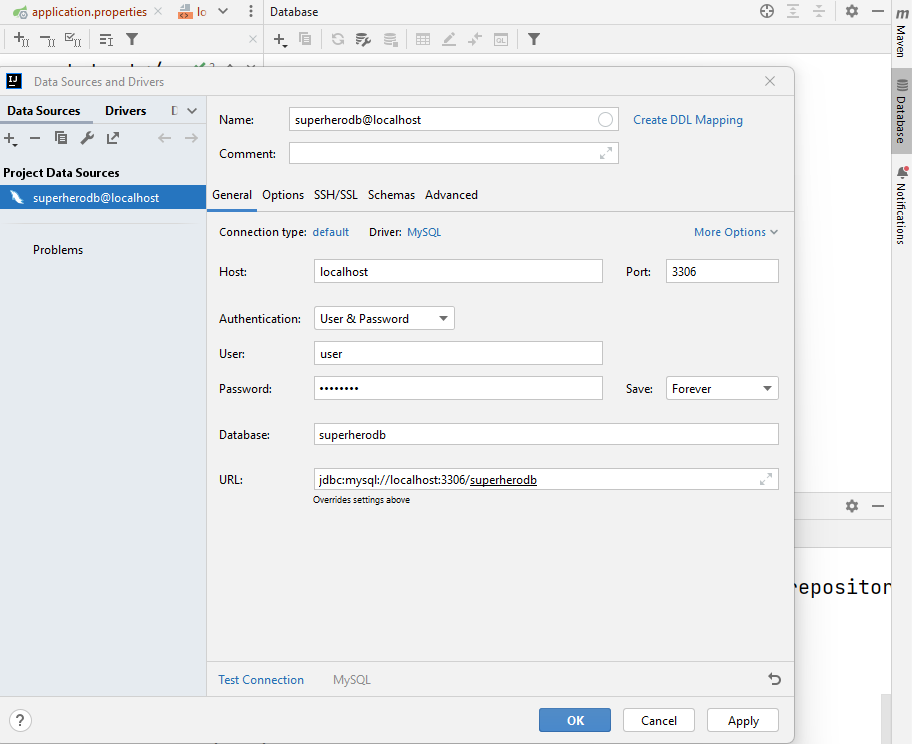
\includegraphics[width=\textwidth]{./images/chapter-jpa/datasource_intellij}}

\frame{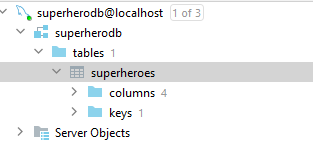
\includegraphics{./images/chapter-jpa/superherodb_localhost}}

\end{oefening}



\section{The Entity class}

\begin{lstlisting}[frame=single,language=java]
package be.pxl.superhero.domain;

import jakarta.persistence.*;
import org.apache.logging.log4j.LogManager;
import org.apache.logging.log4j.Logger;

import java.util.ArrayList;
import java.util.List;

@Entity
@Table(name="superheroes")
public class Superhero {

	private static final Logger LOGGER = LogManager.getLogger(Superhero.class);

	@Id
	@GeneratedValue(strategy = GenerationType.IDENTITY)
	private Long id;
	
	private String firstName;
	private String lastName;
	@Column(unique = true)
	private String superheroName;
	@Column(name="notes")
	private String description;

	public Superhero() {
		// JPA only
	}

	public Superhero(String firstName, String lastName, String superheroName) {
		if (LOGGER.isDebugEnabled()) {
			LOGGER.debug("Creating a new superhero...");
		}
		this.firstName = firstName;
		this.lastName = lastName;
		this.superheroName = superheroName;
	}

	public Long getId() {
		return id;
	}

	public String getFirstName() {
		if (LOGGER.isTraceEnabled()) {
			LOGGER.trace(String.format("FirstName of %s was revealed.", superheroName));
		}
		return firstName;
	}

	public void setFirstName(String firstName) {
		this.firstName = firstName;
	}

	public String getLastName() {
		if (LOGGER.isFatalEnabled()) {
			LOGGER.fatal(String.format("LastName of %s was revealed.", superheroName));
		}
		return lastName;
	}

	public void setLastName(String lastName) {
		this.lastName = lastName;
	}

	public String getSuperheroName() {
		return superheroName;
	}

	public void setSuperheroName(String superheroName) {
		this.superheroName = superheroName;
	}

	@Override
	public String toString() {
		return superheroName;
	}
}
\end{lstlisting}

A JPA entity class is a POJO (Plain Old Java Object) class  that is annotated as having the ability to represent objects in the database.

The \textbf{@Id} annotation marks a field as a primary key field.

The \textbf{@Column} annotation is used to specify the details of the column to which a field or property will be mapped. You can use column annotation with the following most commonly used attributes:
\begin{itemize}
\item \textbf{name}: specify the name of the column.
\item \textbf{length}: specify the size of thee column, particularly for a String value.
\item \textbf{nullable}: mark the column to be NOT NULL when the database schema is generated.
\item \textbf{unique}: mark the column to contain only unique values.
\end{itemize}

\begin{oefening}
$\square$ Create an entity-class Mission.
A mission has following fields:
\begin{tabular}{|c|c|c|}
\hline
id & Long & The primary key.\\
name & String & Unique name of the mission.\\
completed & boolean & \\
deleted & boolean & \\
\hline
\end{tabular}

$\square$ Create MissionRepository, MissionService with MissionServiceImpl and MissionController to make it possible to create, retrieve, update and delete a mission. Add an REST-endpoint to retrieve all missions. Create the necessary DTOs.

\frame{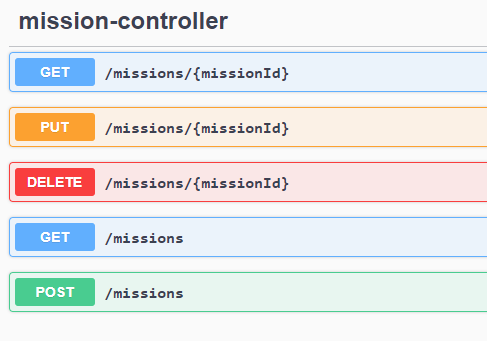
\includegraphics[width=\textwidth]{./images/chapter-jpa/mission_controller}}

\frame{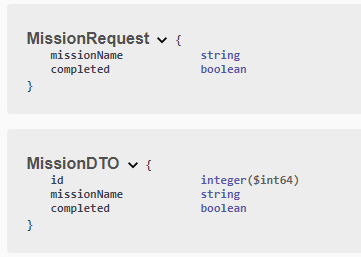
\includegraphics{./images/chapter-jpa/mission_api}}


Test all endpoints manually.

Verify the code quality with SonarQube.
\end{oefening}


\section{Entity lifecycle}

The EntityManager is a core interface of JPA.  An instance of EntityManager is used to create and remove  entity instances, to find entities by their primary key,  and to query over entities.  In fact,  an instance of the EntityManager is used to interact with the persistence context. 

The persistence context is one of the main concepts in JPA.
It is a set of all entity object that you are currently using or used recently. You can think of the persistence context as some kind of first-level cache. Each entity object in the persistence context represents a record in the database.
The persistence context manages these entity objects and their lifecycle. Each entity object has one of 4 states: new, managed, removed, and detached.

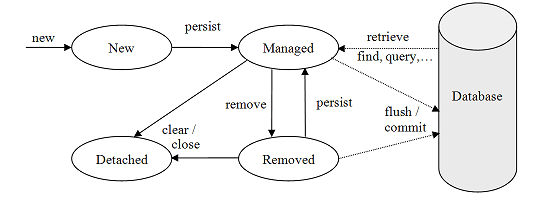
\includegraphics[width=\textwidth]{./images/chapter6/entity_states}

A newly instantiated entity object is in state \textbf{new} or \textbf{transient}. The entity object hasn't been persisted yet, so there's no database record yet. The persistence context does not know about the entity object yet. 

All entity objects that attached to the persistence context are in the lifecycle state \textbf{managed}. An entity object becomes managed when it is persisted to the database. Entity object retrieved from the database are also in the managed state.
If a managed entity object is modified (updated) within an active transaction, the change is detected by the persistence context and passed on to the database.

When a managed entity is removed within an active transaction, the state changes from managed to removed, and the record is physically deleted from the database (when the transaction commits).

An entity gets detached when it is no longer managed by the persistence context but still represents a record in the database.
Detached objects are limited in functionality.


 
Programmatically we need to use the entitymanager to change the state of the entity object in the persistence context which results in changes or updates in our database. 

When using Spring Data JPA you don't have to implement the interaction with the entitymanager. When you create a Repository, the SimpleJpaRepository class provided by Spring Data JPA provides the default implementation. SimpleJpaRepository class internally uses JPA entitymanager.

\begin{oefening}
Open the class SimpleJpaRepository and take a look at its implementation (e.g. save()-method).
\end{oefening}


\section{Queries}

With Spring Data JPA you can create query methods to select records from the database without writing SQL queries. Behind the scenes, Spring Data JPA will create SQL queries based on the query method and execute the query for us.

The query generation from the method name is a query generation strategy where the invoked query is derived from the name of the query method.

Consider a UserRepository with query method findByEmailAddressAndLastname().

\begin{lstlisting}
public interface UserRepository extends JpaRepository<User, Long> {
  List<User> findByEmailAddressAndLastname(String emailAddress, String lastname);
}
\end{lstlisting}

Spring Data JPA behind the scene creates a query which translates into the JPQL query: select u from User u where u.emailAddress = ?1 and u.lastname = ?2. 

\begin{oefening}
In the interface SuperheroRepository you add a method for retrieving a Superhero by its Supheroname. The method should an Optional.
\end{oefening}


\section{Unit testing a repository}

Spring Data JPA offers an annotation @DataJpaTest which makes repository testing possible with a minimum of configuration. 


\begin{lstlisting}[frame=single, language=java]
package be.pxl.superhero.repository;

import be.pxl.superhero.builder.SuperheroBuilder;
import be.pxl.superhero.domain.Superhero;
import org.junit.jupiter.api.BeforeEach;
import org.junit.jupiter.api.Test;
import org.springframework.beans.factory.annotation.Autowired;
import org.springframework.boot.test.autoconfigure.orm.jpa.DataJpaTest;

import javax.persistence.EntityManager;
import javax.persistence.PersistenceContext;
import java.util.Optional;

import static org.junit.jupiter.api.Assertions.assertEquals;
import static org.junit.jupiter.api.Assertions.assertTrue;

@DataJpaTest
public class SuperheroRepositoryTest {

	private static final String SUPERHERO_NAME = "Superman";

	@PersistenceContext
	protected EntityManager entityManager;

	@Autowired
	private SuperheroRepository superheroRepository;

	private Superhero superhero = SuperheroBuilder.aSuperhero().withFirstName("Clark").withLastName("Kent").withSuperheroName(SUPERHERO_NAME).build();

	@BeforeEach
	public void init() {
		superheroRepository.save(superhero);
		entityManager.flush();
		entityManager.clear();
	}

	@Test
	public void returnsSuperheroWithGivenSuperheroName() {
		Optional<Superhero> superheroUnderTest = superheroRepository.findSuperheroBySuperheroName(SUPERHERO_NAME);

		assertTrue(superheroUnderTest.isPresent());
		assertEquals(SUPERHERO_NAME, superheroUnderTest.get().getSuperheroName());

	}

	@Test
	public void returnsEmptyOptionalWhenNoInstituteWithGivenName() {
		Optional<Superhero> superheroUnderTest = superheroRepository.findSuperheroBySuperheroName("Robin Hood");

		assertTrue(superheroUnderTest.isEmpty());
	}
}

\end{lstlisting}


\section{Relationships}




